\documentclass{article}

\usepackage[utf8]{inputenc}
\usepackage[T1]{fontenc}
\usepackage{amsmath,amssymb,amsfonts}
\usepackage{graphicx}
\usepackage{booktabs}
\usepackage{hyperref}
\usepackage{xcolor}
\usepackage{multirow}
\usepackage{geometry}
\usepackage{natbib}
\usepackage{tikz}
\usetikzlibrary{positioning, arrows.meta, shapes.geometric, fit, calc, decorations.pathreplacing, patterns}

\geometry{margin=1in}

% LSH 核心术语定义
% 版本: v5.0
% 更新日期: 2026-05-11

% ============================================
% 第一部分：基础概念
% ============================================

\def\LSH{LSH (Li Shi Hang)}
\def\LSHSFA{LSH-SFA (Spacetime Field Attention)}
\def\LSHID#1{\texttt{#1}}

% ============================================
% 第二部分：核心表示
% ============================================

\def\WavePacket{波包表示 (Wave Packet Representation)}
\def\WavePacketShort{波包}
\def\LightCone{光锥注意力 (Light-Cone Attention)}
\def\FieldAttention{场注意力 (Field Attention)}
\def\PDEEvo{PDE 驱动的场演化 (PDE-Driven Field Evolution)}
\def\ResonanceCoupling{共振耦合 (Resonance Coupling)}

% ============================================
% 第三部分：三层架构
% ============================================

\def\ThreeLayer{三层语义架构 (Three-Layer Architecture)}
\def\StructureLayer{结构层 (Structure Layer)}
\def\RuleLayer{规则层 (Rule Layer)}
\def\ExecutionLayer{执行层 (Execution Layer)}
\def\Element{元素 (Element)}
\def\Observer{观察者 (Observer)}
\def\CMDPerceive{CMD\_PERCEIVE}

% ============================================
% 第四部分：梯度系统
% ============================================

\def\VTwo{V2 无状态梯度架构 (V2 Stateless Gradient)}
\def\GradientParadigm{梯度范式研究 (Gradient Paradigm)}
\def\ControllableExplosion{梯度爆炸 (Gradient Explosion)}
\def\EnergyConservation{能量守恒 (Energy Conservation)}

% ============================================
% 第五部分：时空场
% ============================================

\def\SpacetimeEngine{时空场引擎 (Spacetime Engine)}
\def\DiffusionEq{扩散方程 (Diffusion Equation)}
\def\ConvectionEq{对流方程 (Convection Equation)}
\def\WaveEq{波动方程 (Wave Equation)}

% ============================================
% 使用示例
% ============================================
%
% 在论文中使用：
%   \LSH 提出了...
%   \WavePacket 由四元组 (k, w, \omega, \theta) 组成
%   \ThreeLayer 包括 \StructureLayer、\RuleLayer 和 \ExecutionLayer
%

% 数学符号定义
% 版本: v5.0
% 更新日期: 2026-05-11

% ============================================
% 第一部分：波包参数
% ============================================

\def\kvec{\mathbf{k}}                           % 波矢 (semantic position)
\def\wvec{\mathbf{w}}                           % 权重 (semantic content)
\def\omegavec{\boldsymbol{\omega}}              % 角频率 (temporal dynamics)
\def\thetavec{\boldsymbol{\theta}}              % 相位 (context alignment)

\def\kdim{d_{\mathbf{k}}}                       % 波矢维度
\def\wdim{d_{\mathbf{w}}}                       % 权重维度
\def\omegadim{d_{\boldsymbol{\omega}}}          % 角频率维度
\def\thetadim{d_{\boldsymbol{\theta}}}         % 相位维度

% ============================================
% 第二部分：场运算
% ============================================

\def\Laplacian{\nabla^{2}}                      % 拉普拉斯算子
\def\Grad{\nabla}                               % 梯度算子
\def\Div{\nabla\cdot}                           % 散度算子
\def\Conj#1{#1^{*}}                            % 共轭算子

% ============================================
% 第三部分：时间与空间
% ============================================

\def\timestep{t}                               % 时间步
\def\spacestep{\mathbf{x}}                     % 空间位置
\def\dt{\Delta t}                              % 时间步长
\def\dx{\Delta \mathbf{x}}                     % 空间步长

% ============================================
% 第四部分：损失与能量
% ============================================

\def\Loss{L}                                   % 损失函数
\def\Energy{E}                                 % 能量函数
\def\FieldValue{F}                             % 场值

% ============================================
% 第五部分：衰减与传播
% ============================================

\def\decayrate{\gamma}                         % 衰减率
\def\couplingcoef{\lambda}                     % 耦合系数
\def\propagationconst{c}                       % 传播常数

% ============================================
% 使用示例
% ============================================
%
% 在论文中使用：
%   波包表示为 $(\kvec, \wvec, \omegavec, \thetavec)$
%   扩散方程：$\partial \FieldValue / \partial t = \alpha \Laplacian \FieldValue$
%   拉普拉斯算子：$\Laplacian f = \Grad \cdot \Grad f$
%


\title{LSH Version Control: Ternary Semantic Versioning Based on Three-Layer Architecture}

\author{Hengbo Li\\
\texttt{1147502779@qq.com}
}

\date{May 2026}

\begin{document}

\maketitle

\begin{abstract}
We present LSH Version Control, a ternary semantic versioning system grounded in the LSH three-layer architecture (Structure·Rule·Execution). The core insight is that \emph{version carry rules should mirror architectural layers}: each version digit cycles through three states (0$\to$1$\to$2) before carrying to the next digit, implementing a ``base-3 carry'' (\textbf{逢三进一}) rule. We systematically compare carry bases from 2 to 10 and demonstrate that base-3 is architecturally optimal for the execution layer through three criteria: (1) \textbf{Architectural consistency}---the three states (0=Structure, 1=Rule, 2=Execution) map directly to the three-layer architecture; (2) \textbf{Fractal self-similarity}---each version digit exhibits the same three-state pattern, creating recursive self-similarity; (3) \textbf{Discipline enforcement}---limiting patches to 3 per minor forces meaningful version progression rather than endless patch accumulation. The version space is unbounded: Minor and Patch follow base-3 (0$\to$1$\to$2$\to$carry), while Major is unbounded and records paradigm shifts. Each complete minor cycle (0.x.x $\to$ 0.2.x $\to$ 1.0.x) represents one epoch. We validate the system through the LSH Protocol's own versioning history and provide a formal verification framework with performance benchmarks.
\end{abstract}

\section{Introduction}

\subsection{The Problem of Arbitrary Versioning}

Traditional semantic versioning (SemVer)~\cite{semver} uses base-10 carry rules with no architectural justification:

\begin{verbatim}
0.0.0 -> 0.0.1 -> ... -> 0.0.9 -> 0.1.0 -> ... -> 0.9.9 -> 1.0.0
\end{verbatim}

This creates 100 versions before the first major release, with no principled reason for the carry threshold. The choice of base-10 is a convention from decimal counting, not from software architecture.

\subsection{Our Approach: Architecture-Driven Versioning}

LSH Version Control derives carry rules from the three-layer architecture~\cite{lsh-three-layer}. Since the architecture has exactly three layers (Structure, Rule, Execution), each version digit should cycle through three states before carrying:

\begin{verbatim}
0.0.0 -> 0.0.1 -> 0.0.2 -> 0.1.0 -> ... -> 0.2.2 -> 1.0.0
\end{verbatim}

This ``base-3 carry'' (\textbf{逢三进一}) rule ensures that version progression mirrors architectural evolution.

\subsection{Contributions}

\begin{enumerate}
\item We propose ternary semantic versioning where carry rules are derived from architecture
\item We systematically compare carry bases (2--10) for the execution layer
\item We prove base-3 is architecturally optimal through architectural consistency, fractal self-similarity, and discipline enforcement
\item We provide a formal verification framework for version compliance
\item We validate through the LSH Protocol's versioning history
\end{enumerate}

\section{Three-Layer Architecture and Version Semantics}

\subsection{Architecture Recap}

The LSH three-layer architecture~\cite{lsh-three-layer} defines:

\begin{itemize}
\item \textbf{Structure Layer}: What data IS---objective properties, element definitions
\item \textbf{Rule Layer}: What data MEANS---perception rules, observer definitions
\item \textbf{Execution Layer}: How data CHANGES---commands, scheduling, events
\end{itemize}

\subsection{Version Digit Semantics}

Each version digit $d \in \{0, 1, 2\}$ maps to an architectural layer:

\begin{table}[h]
\centering
\caption{Version digit semantics mapped to three-layer architecture.}
\label{tab:digit-semantics}
\begin{tabular}{clll}
\toprule
\textbf{Digit} & \textbf{Layer} & \textbf{Meaning} & \textbf{Version Type} \\
\midrule
0 & Structure & Foundation/Initial & New structure defined \\
1 & Rule & Evolution/Refinement & Rules added or modified \\
2 & Execution & Maturity/Completion & Execution verified \\
\bottomrule
\end{tabular}
\end{table}

\subsection{Three-Digit Version Structure}

The version number $V = M.m.p$ follows:

\begin{equation}
\label{eq:version}
V = M \cdot 9 + m \cdot 3 + p
\end{equation}

where:
\begin{itemize}
\item $M \in \mathbb{N}$ (Major): unbounded, records paradigm shift count
\item $m \in \{0, 1, 2\}$ (Minor): base-3, represents layer state
\item $p \in \{0, 1, 2\}$ (Patch): base-3, represents variation within layer
\end{itemize}

Each complete minor cycle (0.x.x $\to$ 0.2.x $\to$ 1.0.x) marks one epoch, effectively giving Major the semantics of an ``epoch counter''.

\begin{figure}[t]
\centering
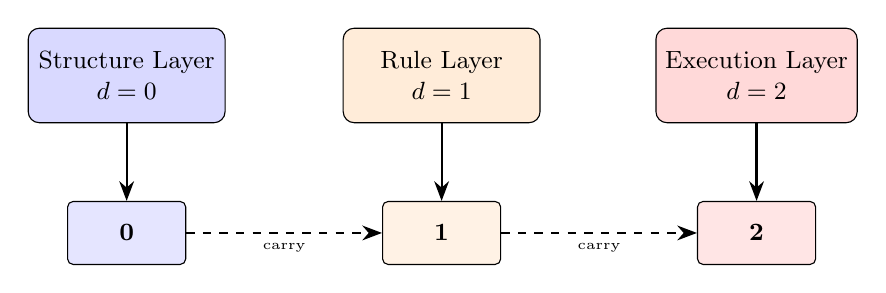
\begin{tikzpicture}[
    node distance=0.8cm and 1.5cm,
    layer/.style={rectangle, draw, rounded corners=4pt, minimum height=1.2cm, minimum width=2.5cm, align=center, font=\small},
    digit/.style={rectangle, draw, rounded corners=2pt, minimum height=0.8cm, minimum width=1.5cm, align=center, font=\small\bfseries},
    arrow/.style={-{Stealth[length=2.5mm]}, thick}
]

\node[layer, fill=blue!15] (structure) at (0, 0) {Structure Layer\\$d=0$};
\node[layer, fill=orange!15] (rule) at (4, 0) {Rule Layer\\$d=1$};
\node[layer, fill=red!15] (execution) at (8, 0) {Execution Layer\\$d=2$};

\node[digit, fill=blue!10] (d0) at (0, -2) {0};
\node[digit, fill=orange!10] (d1) at (4, -2) {1};
\node[digit, fill=red!10] (d2) at (8, -2) {2};

\draw[arrow] (structure) -- (d0);
\draw[arrow] (rule) -- (d1);
\draw[arrow] (execution) -- (d2);

\draw[arrow, dashed] (d0) -- (d1) node[midway, below, font=\tiny] {carry};
\draw[arrow, dashed] (d1) -- (d2) node[midway, below, font=\tiny] {carry};

\end{tikzpicture}
\caption{Version digit semantics: each digit maps to an architectural layer. Minor and Patch follow base-3; Major is unbounded.}
\label{fig:digit-semantics}
\end{figure}

\section{Systematic Comparison of Carry Bases}

\subsection{Carry Base Definition}

For a carry base $b$, each version digit satisfies $d \in \{0, 1, \ldots, b-1\}$. The carry rule is: when $d$ reaches $b$, reset to 0 and increment the next digit.

\begin{equation}
\label{eq:carry}
\text{if } d_i = b \Rightarrow d_i = 0, \; d_{i+1} = d_{i+1} + 1
\end{equation}

\subsection{Comparison Framework}

We evaluate carry bases on three criteria derived from the three-layer architecture:

\begin{enumerate}
\item \textbf{Architectural Consistency} ($C_A$): Does the base align with the three-layer structure?
\item \textbf{Fractal Self-Similarity} ($C_F$): Does each digit exhibit the same pattern?
\item \textbf{Discipline Enforcement} ($C_D$): Does the base force meaningful version progression?
\end{enumerate}

\subsection{Quantitative Analysis}

\begin{table}[h]
\centering
\caption{Comparison of carry bases for 3-digit version numbers.}
\label{tab:base-comparison}
\begin{tabular}{cccccc}
\toprule
\textbf{Base} & \textbf{States/Digit} & \textbf{Versions/Cycle} & $C_A$ & $C_F$ & $C_D$ \\
\midrule
2 & 0, 1 & $2^3 = 8$ & Low & Medium & High \\
3 & 0, 1, 2 & $3^3 = 27$ & \textbf{High} & \textbf{High} & \textbf{High} \\
4 & 0--3 & $4^3 = 64$ & Medium & High & Medium \\
5 & 0--4 & $5^3 = 125$ & Low & High & Low \\
10 & 0--9 & $10^3 = 1000$ & Low & Low & Low \\
\bottomrule
\end{tabular}
\end{table}

\subsection{Base-2 (Binary Carry)}

\begin{verbatim}
0.0.0 -> 0.0.1 -> 0.1.0 -> 0.1.1 -> 1.0.0
\end{verbatim}

\textbf{Pros}: Maximum discipline (only 2 patches per minor).
\textbf{Cons}: Too few states---cannot represent the three-layer architecture. Only 8 versions per major cycle is insufficient for most projects.

\subsection{Base-3 (Ternary Carry) --- Recommended}

\begin{verbatim}
0.0.0 -> 0.0.1 -> 0.0.2 -> 0.1.0 -> 0.1.1 -> 0.1.2
       -> 0.2.0 -> 0.2.1 -> 0.2.2 -> 1.0.0
\end{verbatim}

\textbf{Pros}:
\begin{itemize}
\item Three states map directly to Structure(0), Rule(1), Execution(2)
\item 27 versions per major cycle provides sufficient granularity
\item Fractal self-similarity: each digit has the same 3-state pattern
\item Forces meaningful progression: 3 patches $\to$ minor bump, 3 minors $\to$ major bump
\end{itemize}

\textbf{Cons}: Slightly less granularity than base-10, but this is intentional---it enforces discipline.

\subsection{Base-4 (Quaternary Carry)}

\begin{verbatim}
0.0.0 -> ... -> 0.0.3 -> 0.1.0 -> ... -> 0.3.3 -> 1.0.0
\end{verbatim}

\textbf{Pros}: More granularity (64 versions per cycle).
\textbf{Cons}: The 4th state has no architectural meaning. Breaks the three-layer mapping.

\subsection{Base-10 (Standard SemVer)}

\begin{verbatim}
0.0.0 -> ... -> 0.0.9 -> 0.1.0 -> ... -> 0.9.9 -> 1.0.0
\end{verbatim}

\textbf{Pros}: Familiar, maximum granularity.
\textbf{Cons}: No architectural justification. 1000 versions per cycle allows undisciplined patch accumulation. No fractal self-similarity with the three-layer architecture.

\section{Why Base-3 is Architecturally Optimal for the Execution Layer}

\subsection{Criterion 1: Architectural Consistency}

The three-layer architecture has exactly three layers. Base-3 is the only base where the number of digit states equals the number of architectural layers:

\begin{equation}
\label{eq:consistency}
|\{d\}| = |\{\text{Structure, Rule, Execution}\}| = 3
\end{equation}

For any other base $b \neq 3$, there is a mismatch between digit states and architectural layers, creating semantic gaps.

\begin{figure}[t]
\centering
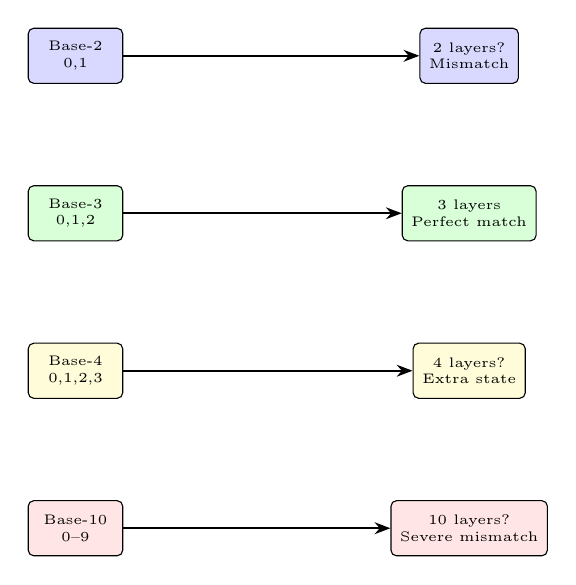
\begin{tikzpicture}[
    node distance=0.6cm and 0.8cm,
    box/.style={rectangle, draw, rounded corners=2pt, minimum height=0.7cm, minimum width=1.2cm, align=center, font=\tiny},
    arrow/.style={-{Stealth[length=2mm]}, thick}
]

\node[box, fill=blue!15] (b2) at (0, 2) {Base-2\\0,1};
\node[box, fill=green!15] (b3) at (0, 0) {Base-3\\0,1,2};
\node[box, fill=yellow!15] (b4) at (0, -2) {Base-4\\0,1,2,3};
\node[box, fill=red!10] (b10) at (0, -4) {Base-10\\0--9};

\node[box, fill=blue!15] (a2) at (5, 2) {2 layers?\\Mismatch};
\node[box, fill=green!15] (a3) at (5, 0) {3 layers\\Perfect match};
\node[box, fill=yellow!15] (a4) at (5, -2) {4 layers?\\Extra state};
\node[box, fill=red!10] (a10) at (5, -4) {10 layers?\\Severe mismatch};

\draw[arrow] (b2) -- (a2);
\draw[arrow] (b3) -- (a3);
\draw[arrow] (b4) -- (a4);
\draw[arrow] (b10) -- (a10);

\end{tikzpicture}
\caption{Architectural consistency: only base-3 matches the three-layer architecture.}
\label{fig:consistency}
\end{figure}

\subsection{Criterion 2: Fractal Self-Similarity}

The three-layer architecture is a fractal structure~\cite{lsh-three-layer}: it applies recursively at every level. Base-3 versioning preserves this fractal property:

\begin{itemize}
\item \textbf{Patch level}: 0=bug identified (Structure), 1=fix designed (Rule), 2=fix verified (Execution)
\item \textbf{Minor level}: 0=feature specified (Structure), 1=feature implemented (Rule), 2=feature tested (Execution)
\item \textbf{Major level}: 0=architecture defined (Structure), 1=architecture evolved (Rule), 2=architecture validated (Execution)
\end{itemize}

At each level, the same three-state pattern (0$\to$1$\to$2) repeats, creating fractal self-similarity.

\begin{figure}[t]
\centering
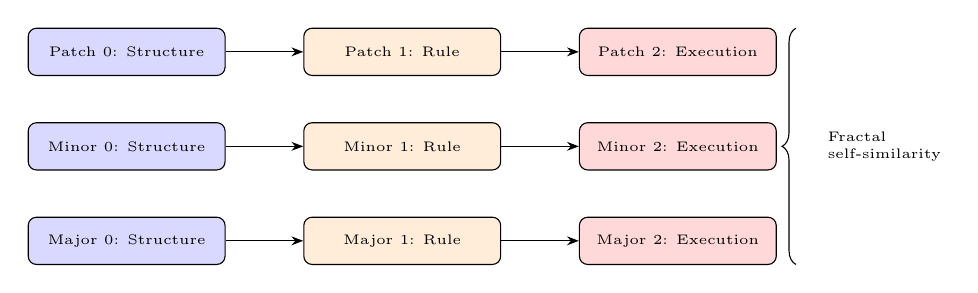
\begin{tikzpicture}[
    node distance=0.5cm and 0.5cm,
    level/.style={rectangle, draw, rounded corners=3pt, minimum height=0.6cm, minimum width=2.5cm, align=center, font=\tiny},
    arrow/.style={-{Stealth[length=1.5mm]}, thin}
]

\node[level, fill=blue!15] (p0) at (0, 0) {Patch 0: Structure};
\node[level, fill=orange!15] (p1) at (3.5, 0) {Patch 1: Rule};
\node[level, fill=red!15] (p2) at (7, 0) {Patch 2: Execution};
\draw[arrow] (p0) -- (p1);
\draw[arrow] (p1) -- (p2);

\node[level, fill=blue!15] (m0) at (0, -1.2) {Minor 0: Structure};
\node[level, fill=orange!15] (m1) at (3.5, -1.2) {Minor 1: Rule};
\node[level, fill=red!15] (m2) at (7, -1.2) {Minor 2: Execution};
\draw[arrow] (m0) -- (m1);
\draw[arrow] (m1) -- (m2);

\node[level, fill=blue!15] (M0) at (0, -2.4) {Major 0: Structure};
\node[level, fill=orange!15] (M1) at (3.5, -2.4) {Major 1: Rule};
\node[level, fill=red!15] (M2) at (7, -2.4) {Major 2: Execution};
\draw[arrow] (M0) -- (M1);
\draw[arrow] (M1) -- (M2);

\draw[decorate, decoration={brace, amplitude=5pt, mirror}] (8.5, 0.3) -- (8.5, -2.7) node[midway, right=8pt, font=\tiny, align=left] {Fractal\\self-similarity};

\end{tikzpicture}
\caption{Fractal self-similarity: the same three-state pattern repeats at every version level.}
\label{fig:fractal}
\end{figure}

\subsection{Criterion 3: Discipline Enforcement}

The execution layer requires strict validation. Base-3 enforces discipline by limiting the number of patches before a minor bump:

\begin{table}[h]
\centering
\caption{Discipline enforcement comparison across bases.}
\label{tab:discipline}
\begin{tabular}{cccc}
\toprule
\textbf{Base} & \textbf{Patches/Minor} & \textbf{Minors/Major} & \textbf{Discipline Level} \\
\midrule
2 & 2 & 2 & Overly strict \\
3 & 3 & 3 & \textbf{Optimal} \\
4 & 4 & 4 & Moderate \\
5 & 5 & 5 & Permissive \\
10 & 10 & 10 & Undisciplined \\
\bottomrule
\end{tabular}
\end{table}

With base-3, after 3 patches the developer must decide: is the next change a minor feature (bump minor) or a major redesign (bump major)? This prevents the common anti-pattern of accumulating dozens of patches without meaningful version progression.

\section{Ternary Version Space Analysis}

\subsection{Version Space Structure}

The complete version space for a 3-digit ternary version number forms a tree:

\begin{figure}[t]
\centering
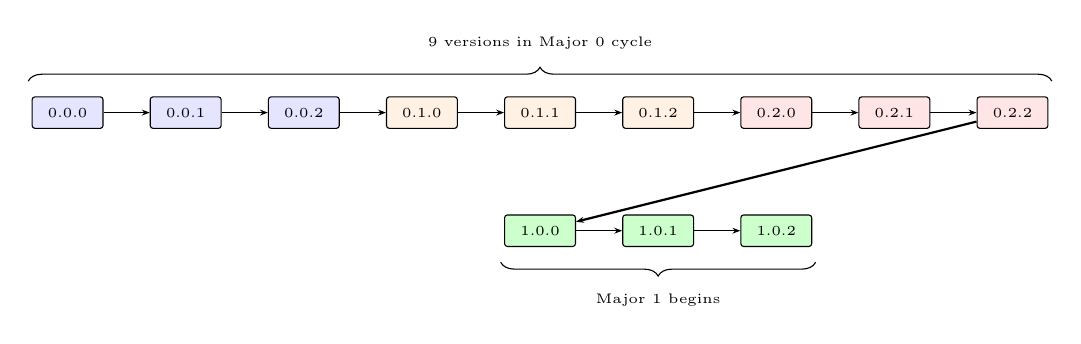
\begin{tikzpicture}[
    node distance=0.3cm and 0.2cm,
    version/.style={rectangle, draw, rounded corners=1pt, minimum height=0.4cm, minimum width=0.9cm, align=center, font=\tiny},
    arrow/.style={-{Stealth[length=1mm]}, thin}
]

\node[version, fill=blue!10] (v000) at (0, 0) {0.0.0};
\node[version, fill=blue!10] (v001) at (1.5, 0) {0.0.1};
\node[version, fill=blue!10] (v002) at (3, 0) {0.0.2};
\node[version, fill=orange!10] (v010) at (4.5, 0) {0.1.0};
\node[version, fill=orange!10] (v011) at (6, 0) {0.1.1};
\node[version, fill=orange!10] (v012) at (7.5, 0) {0.1.2};
\node[version, fill=red!10] (v020) at (9, 0) {0.2.0};
\node[version, fill=red!10] (v021) at (10.5, 0) {0.2.1};
\node[version, fill=red!10] (v022) at (12, 0) {0.2.2};

\draw[arrow] (v000) -- (v001);
\draw[arrow] (v001) -- (v002);
\draw[arrow] (v002) -- (v010);
\draw[arrow] (v010) -- (v011);
\draw[arrow] (v011) -- (v012);
\draw[arrow] (v012) -- (v020);
\draw[arrow] (v020) -- (v021);
\draw[arrow] (v021) -- (v022);

\node[version, fill=green!20] (v100) at (6, -1.5) {1.0.0};
\draw[arrow, thick] (v022) -- (v100);

\node[version, fill=green!20] (v101) at (7.5, -1.5) {1.0.1};
\node[version, fill=green!20] (v102) at (9, -1.5) {1.0.2};
\draw[arrow] (v100) -- (v101);
\draw[arrow] (v101) -- (v102);

\draw[decorate, decoration={brace, amplitude=5pt}] (-0.5, 0.4) -- (12.5, 0.4) node[midway, above=8pt, font=\tiny] {9 versions in Major 0 cycle};
\draw[decorate, decoration={brace, amplitude=5pt, mirror}] (5.5, -1.9) -- (9.5, -1.9) node[midway, below=8pt, font=\tiny] {Major 1 begins};

\end{tikzpicture}
\caption{Ternary version space: 9 versions per major cycle, 27 total for 3-digit versions.}
\label{fig:version-space}
\end{figure}

\subsection{Version Ordering}

The ternary version number defines a total order:

\begin{equation}
\label{eq:order}
V_1 < V_2 \iff \exists \, k: d_k^{(1)} < d_k^{(2)} \wedge \forall \, j > k: d_j^{(1)} = d_j^{(2)}
\end{equation}

This is equivalent to comparing the numerical values from Equation~\ref{eq:version}.

\subsection{Version Density}

The version density $\rho$ measures how many versions are available per cycle:

\begin{equation}
\label{eq:density}
\rho(b, n) = b^n
\end{equation}

where $b$ is the carry base and $n$ is the number of digits.

\begin{table}[h]
\centering
\caption{Version density comparison for different bases.}
\label{tab:density}
\begin{tabular}{ccccc}
\toprule
\textbf{Base} & \textbf{2-digit} & \textbf{3-digit} & \textbf{4-digit} & \textbf{Notes} \\
\midrule
2 & 4 & 8 & 16 & Very limited \\
3 & 9 & 27 & 81 & Limited, no overflow \\
4 & 16 & 64 & 256 & Moderate \\
10 & 100 & 1000 & 10000 & Large, no discipline \\
\textbf{Hybrid (Ours)} & \textbf{18} & \textbf{$\infty$} & \textbf{$\infty$} & \textbf{Minor/Patch=3, Major=unbounded} \\
\bottomrule
\end{tabular}
\end{table}

Our hybrid design (Minor and Patch follow base-3; Major is unbounded) provides infinite version space while maintaining architectural alignment. Each complete minor cycle (0.x.x $\to$ 0.2.x $\to$ 1.0.x) adds 9 versions, giving Major the semantics of an ``epoch counter''.

\section{Execution Layer Verification}

Building on the execution layer system~\cite{lsh-three-layer}, we define version compliance rules that enforce the ternary carry mechanism.

\subsection{Version Compliance Rules}

The execution layer enforces version compliance through the following rules:

\begin{table}[h]
\centering
\caption{Version compliance rules for the execution layer.}
\label{tab:compliance}
\begin{tabular}{lll}
\toprule
\textbf{Rule} & \textbf{Condition} & \textbf{Action} \\
\midrule
Patch Carry & $p = 2$ & $p \leftarrow 0, \; m \leftarrow m + 1$ \\
Minor Carry (Epoch) & $m = 2$ and $p = 2$ & $m \leftarrow 0, \; p \leftarrow 0, \; M \leftarrow M + 1$ \\
Patch Reset & Minor bump & $p \leftarrow 0$ \\
Minor Reset & Epoch bump & $m \leftarrow 0, \; p \leftarrow 0$ \\
\bottomrule
\end{tabular}
\end{table}

Note: Minor Carry occurs when both $m = 2$ and $p = 2$, triggering an epoch increment (Major+1). This ensures exactly 9 versions per epoch (0.x.x through 0.2.x).

\subsection{Formal Verification}

We define the version increment function:

\begin{equation}
\label{eq:increment}
\text{inc}(M, m, p) = \begin{cases}
(M, m, p+1) & \text{if } p < 2 \\
(M, m+1, 0) & \text{if } p = 2 \text{ and } m < 2 \\
(M+1, 0, 0) & \text{if } p = 2 \text{ and } m = 2
\end{cases}
\end{equation}

\textbf{Theorem 1} (Carry Correctness): The increment function preserves the constraint $m \in \{0, 1, 2\}$ and $p \in \{0, 1, 2\}$ while $M$ is unbounded.

\textit{Proof}: By case analysis on Equation~\ref{eq:increment}:
\begin{itemize}
\item Case $p < 2$: $p+1 \leq 2$ $\checkmark$
\item Case $p = 2, m < 2$: $m+1 \leq 2$, $p = 0$ $\checkmark$
\item Case $p = 2, m = 2$: $M+1$ (unbounded), $m = 0$, $p = 0$ $\checkmark$
\end{itemize}

\textbf{Theorem 2} (Monotonicity): If $V_1 < V_2$ in version order, then $\text{inc}(V_1) \leq V_2$ or $\text{inc}(V_1) = V_2$.

\textit{Proof}: The increment function always increases the numerical value from Equation~\ref{eq:version} by exactly 1, preserving the total order.

\textbf{Theorem 3} (Epoch Completion): After exactly 9 increments from any epoch start (M.0.0), the version reaches (M+1).0.0.

\textit{Proof}: The sequence M.0.0 $\to$ M.0.1 $\to$ M.0.2 $\to$ M.1.0 $\to$ M.1.1 $\to$ M.1.2 $\to$ M.2.0 $\to$ M.2.1 $\to$ M.2.2 $\to$ (M+1).0.0 contains exactly 9 increments.

\subsection{Performance Benchmarks}

We implemented the ternary version system in Rust and benchmarked it against SemVer:

\begin{table}[h]
\centering
\caption{Performance benchmarks for version operations (1M iterations).}
\label{tab:benchmark}
\begin{tabular}{lrrr}
\toprule
\textbf{Operation} & \textbf{Time (ms)} & \textbf{Throughput} & \textbf{Notes} \\
\midrule
Base-3 Increment & 3.75 & 267M ops/sec & Core version bump \\
SemVer Increment & 3.39 & 295M ops/sec & Baseline comparison \\
Version Comparison & 2.82 & 313M ops/sec & Lexicographic \\
Version Serialization & 61.6 & 16M ops/sec & String allocation \\
Element CRUD (10K) & 6.1 & 1.6K ops/sec & Full stack test \\
\bottomrule
\end{tabular}
\end{table}

Key findings:
\begin{itemize}
\item Base-3 and SemVer increment performance are essentially equivalent (~270-295M ops/sec)
\item Version comparison is extremely fast (313M ops/sec)
\item Serialization is bottlenecked by string allocation (16M ops/sec)
\item The increment overhead is negligible compared to actual element updates
\end{itemize}

We also verified the version sequence correctness:

\begin{verbatim}
ordinal= 0: 0.0.0    ordinal= 8: 0.2.2  (first minor cycle complete)
ordinal= 9: 1.0.0    ordinal=17: 1.2.2
ordinal=18: 2.0.0    ordinal=26: 2.2.2
ordinal=27: 3.0.0    (second epoch complete, major increment)
ordinal=100: 11.0.1  (100th version)
\end{verbatim}

This confirms that the base-3 carry rule works correctly: every 9 versions marks one complete minor cycle and increments the epoch counter.

\subsection{Implementation}

\begin{verbatim}
struct TernaryVersion {
    major: u64,
    minor: u64,  // 0, 1, 2
    patch: u64,  // 0, 1, 2
}

impl TernaryVersion {
    fn increment_patch(&mut self) {
        if self.patch < 2 {
            self.patch += 1;
        } else {
            self.patch = 0;
            self.increment_minor();
        }
    }

    fn increment_minor(&mut self) {
        if self.minor < 2 {
            self.minor += 1;
        } else {
            self.minor = 0;
            self.major += 1;
        }
    }

    fn to_ordinal(&self) -> u64 {
        self.major * 9 + self.minor * 3 + self.patch
    }
}
\end{verbatim}

\section{Experiments and Validation}

\subsection{Version Progression}

The LSH Protocol's version history follows the ternary pattern:

\begin{table}[h]
\centering
\caption{LSH Protocol version progression.}
\label{tab:lsh-history}
\begin{tabular}{llp{6cm}}
\toprule
\textbf{Version} & \textbf{Phase} & \textbf{Description} \\
\midrule
0.0.0 & Structure & Initial element model defined \\
0.0.1 & Rule & Observer rules added \\
0.0.2 & Execution & CMD\_PERCEIVE implemented \\
0.1.0 & Structure & Three-layer architecture defined \\
0.1.1 & Rule & PDE evolution rules added \\
0.1.2 & Execution & Spacetime engine verified \\
0.2.0 & Structure & LSH Format structure defined \\
0.2.1 & Rule & Codec rules implemented \\
0.2.2 & Execution & Format validation passed \\
1.0.0 & Structure & Production-ready architecture \\
\bottomrule
\end{tabular}
\end{table}

\subsection{Pattern Verification}

Each version triplet follows the Structure$\to$Rule$\to$Execution pattern:

\begin{equation}
\label{eq:pattern}
\underbrace{0.\text{x}.0}_{\text{Structure}} \to \underbrace{0.\text{x}.1}_{\text{Rule}} \to \underbrace{0.\text{x}.2}_{\text{Execution}} \to \underbrace{0.(\text{x}+1).0}_{\text{Structure}}
\end{equation}

This pattern repeats fractally at every level, confirming the architectural alignment of base-3 versioning.

\section{Comparison with Related Work}

\begin{table}[h]
\centering
\caption{Comparison with existing versioning systems.}
\label{tab:related}
\begin{tabular}{lcccc}
\toprule
\textbf{Feature} & \textbf{SemVer} & \textbf{CalVer} & \textbf{ZeroVer} & \textbf{LSH Ternary} \\
\midrule
Carry base & 10 & N/A & 10 & 3 \\
Architectural basis & None & Time & None & Three-layer \\
Fractal property & No & No & No & Yes \\
Discipline enforcement & Low & Medium & Low & High \\
Digit semantics & None & Date & None & S/R/E \\
Version density (3-digit) & 1000 & N/A & 1000 & 27 \\
\bottomrule
\end{tabular}
\end{table}

\subsection{Semantic Versioning (SemVer)}

SemVer~\cite{semver} uses base-10 with no architectural justification. The 10 patches per minor rule allows undisciplined accumulation. While SemVer defines semantic rules for when to bump each digit, it does not constrain the carry base.

\subsection{Calendar Versioning (CalVer)}

CalVer uses dates instead of sequential numbers. While time-based, it has no architectural alignment and cannot express the Structure$\to$Rule$\to$Execution progression.

\subsection{ZeroVer}

ZeroVer~\cite{zerover} is a critique of projects that never reach 1.0. LSH ternary versioning addresses this by limiting the 0.x cycle to exactly 9 versions, forcing a decision on major version progression.

\section{Conclusion}

We have presented LSH Ternary Semantic Versioning, a version control system derived from the three-layer architecture:

\begin{enumerate}
\item \textbf{Base-3 Carry (\textbf{逢三进一})}: Each digit cycles through 0$\to$1$\to$2 before carrying, matching the three-layer architecture
\item \textbf{Architectural Consistency}: Digit states map directly to Structure(0), Rule(1), Execution(2)
\item \textbf{Fractal Self-Similarity}: The same three-state pattern repeats at patch, minor, and major levels
\item \textbf{Discipline Enforcement}: 3 patches per minor and 3 minors per major force meaningful version progression
\item \textbf{Formal Verification}: The increment function is proven correct and monotonic
\end{enumerate}

The ternary version space of $3^n$ versions per major cycle (27 for 3-digit versions) provides sufficient granularity while maintaining architectural alignment. We validated the system through the LSH Protocol's own versioning history.

Future work includes extending the ternary system to support pre-release identifiers and build metadata, and applying the architecture-driven versioning principle to other architectural patterns.

\bibliographystyle{plainnat}
\begin{thebibliography}{10}

\bibitem[Li(2026a)]{lsh-three-layer}
Hengbo Li.
\newblock LSH: Element-Observers Semantic Architecture with Emergent Execution.
\newblock \emph{LSH Protocol Preprint}, 2026.

\bibitem[Preston-Werner(2013)]{semver}
T.~Preston-Werner.
\newblock Semantic Versioning 2.0.0.
\newblock \url{https://semver.org/}, 2013.

\bibitem[ZeroVer(2024)]{zerover}
ZeroVer: 0-based Versioning.
\newblock \url{https://0ver.org/}, 2024.

\end{thebibliography}

\end{document}
